Given,
\begin{align}
\vec{x}^T\myvec{1 & 0\\0 & -1}\vec{x}+2\myvec{-2 & -3}\vec{x}-6=0\label{eq:solutions/3/4/1/given}
\intertext{where}
\vec{V}=\myvec{1 & 0 \\0 & -1}\\
\vec{u}=\myvec{-2 \\ -3}
\end{align}
Origin which is moved to the point is given by
\begin{align}
\vec{c}&=\myvec{2\\-3}
\end{align}
The above equation \eqref{eq:solutions/3/4/1/given} can be modified as 
\begin{align}
(\vec{x}+\vec{c})^T\vec{V}(\vec{x}+\vec{c})+2\vec{u}^T(\vec{x}+\vec{c})-6&=0\label{eq:solutions/3/4/1/finalsub}
\end{align}
From equation \eqref{eq:solutions/3/4/1/finalsub} consider,
\begin{align}
    &\implies(\vec{x}+\vec{c})^T\vec{V}(\vec{x}+\vec{c})\\
    &\implies\vec{x}^T\vec{V}\vec{x}+\vec{c}^T\vec{V}\vec{x}+\vec{x}^T\vec{V}\vec{c}+\vec{c}^T\vec{V}\vec{c}\label{eq:solutions/3/4/1/1n}\\
    \intertext{we know that}
    &\vec{x}^T\vec{V}\vec{c}=\vec{c}^T\vec{V}\vec{x}\label{eq:solutions/3/4/1/p}
    \intertext{Substituting equation \eqref{eq:solutions/3/4/1/p} in equation \eqref{eq:solutions/3/4/1/1n}}
    &\implies\vec{x}^T\vec{V}\vec{x}+2\vec{c}^T\vec{V}\vec{x}+\vec{c}^T\vec{V}\vec{c}\label{eq:solutions/3/4/1/eq1}
\end{align}
\begin{align}
    \vec{c}^T\vec{V}\vec{x}&=\myvec{2&-3}\myvec{1&0\\0&-1}\vec{x}=\myvec{2&3}\vec{x}\label{eq:solutions/3/4/1/1.1}\\
    \vec{c}^T\vec{V}\vec{c}&=\myvec{2&-3}\myvec{1&0\\0&-1}\myvec{2\\-3}=-5\label{eq:solutions/3/4/1/1.3}
\end{align}
Substituting the equations \eqref{eq:solutions/3/4/1/1.1}, \eqref{eq:solutions/3/4/1/1.3} in equation \eqref{eq:solutions/3/4/1/eq1} we get 
\begin{align}
    &\implies\vec{x}^T\myvec{1&0\\0&-1}\vec{x}+2\myvec{2&3}\vec{x}-5\label{eq:solutions/3/4/1/1f}
\end{align}
From equation \eqref{eq:solutions/3/4/1/finalsub} consider,
\begin{align}
&\implies 2\vec{u}^T(\vec{x}+\vec{c})\\
&\implies 2\myvec{-2 & -3}\vec{x}+2\myvec{-2 & -3}\myvec{2\\ -3}\\
&\implies -2\myvec{2&3}\vec{x}+10\label{eq:solutions/3/4/1/2f}
\end{align}

Substituting equations \eqref{eq:solutions/3/4/1/1f}, \eqref{eq:solutions/3/4/1/2f} in equation \eqref{eq:solutions/3/4/1/finalsub} we get 
\begin{align}
    \vec{x}^T\myvec{1&0\\0&-1}\vec{x}+2\myvec{2&3}\vec{x}-2\myvec{2&3}\vec{x}+10-11&=0
\end{align}
\begin{align}
    \implies\vec{x}^T\myvec{1&0\\0&-1}\vec{x}-1&=0\label{eq:solutions/3/4/1/result}
\end{align}
Given equation \eqref{eq:solutions/3/4/1/given} is modified to equation \eqref{eq:solutions/3/4/1/result} when the origin is moved to the point $\myvec{2\\-3}$ which is verified through the plot \ref{eq:solutions/3/4/1/Fig :1}

From equations \eqref{eq:solutions/3/4/1/result} ,\eqref{eq:solutions/3/4/1/given} $\vec{V}$ doesn't change
\begin{align}
    \det(\vec{V})&=-1
\end{align}
Since $\det(\vec{V})<0$ the given equation represents the hyperbola

\begin{figure}[h]
    \centering
    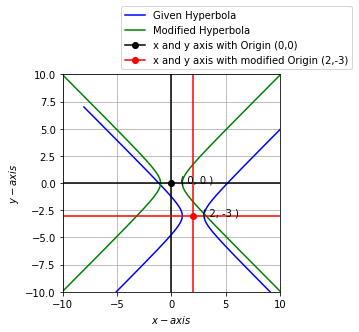
\includegraphics[width=\columnwidth]{./solutions/3/4/1/Assignment 7.png}
    \caption{Hyperbola when origin is shifted}
    \label{eq:solutions/3/4/1/Fig :1}
\end{figure}

The plot \ref{eq:solutions/3/4/1/Fig :1} verifies the given hyperbola
\begin{align}
\vec{x}^T\myvec{1 & 0\\0 & -1}\vec{x}-\myvec{4 & 6}\vec{x}-6=0
\end{align}
The above hyperbola was plotted with respect to origin with
\begin{align}
    \intertext{centre,} 
    \vec{c_1}&=\myvec{2\\-3} 
    \intertext{vertices,} 
    \vec{v_{11}}&=\myvec{3\\-3}\\
    \vec{v_{12}}&=\myvec{1\\-3}
\end{align} 
The given hyperbola equation \eqref{eq:solutions/3/4/1/given} which is modified to the hyperbola
\begin{align}
    \vec{x}^T\myvec{1&0\\0&-1}\vec{x}-1=0
    \intertext{centre,}
    \vec{c_2}=\myvec{0\\0}
    \intertext{vertices}
    \vec{v_{21}}&=\myvec{1\\0}\\
    \vec{v_{22}}&=\myvec{-1\\0}
    \intertext{when the origin is moved to the point}
    \vec{o}&=\myvec{2\\-3}
\end{align} 
